%TD n o 6
\chapter{Échanges entre particules et champ électromagnétique}
\section{Échange d'impulsion entre particules et champ électromagnétique}%1
\begin{minipage}[c]{.65\linewidth}
\hspace{0.5cm}Considérons l'expérience schématisée sur la figure ci-contre. Une particule de masse $m$ , de charge $q$ initialement au repos, est placée à une
distance $b$ d'un solenoïde infiniment long, de rayon $a$ , comportant $n$ spires
par mètre et parcouru par un courant constant $I$.

\hspace{0.5cm}On rappelle les expressions des champs {\bf A} et {\bf B} pour une telle distribution
de courant à l'intérieur et à l'extérieur du solenoïde :
\[
{\bf B} =\left\{
  \begin{array}{lcr}
   0 &  & \tx{si}\ r > a \\
   \mu_0nI {\bf e}_z &  & \tx{si}\ r < a \\
  \end{array}
\right.\]
\[
{\bf A} =\left\{
  \begin{array}{lcr}
 \frac{Ba^2}{2r} {\bf e}_\theta &  & \tx{si}\ r > a \\
 \frac{Br}{2} {\bf e}_\theta &  & \tx{si}\ r < a \\
  \end{array}
\right.\]
\end{minipage}
\hfill
\begin{minipage}[c]{.25\linewidth}
\begin{center}
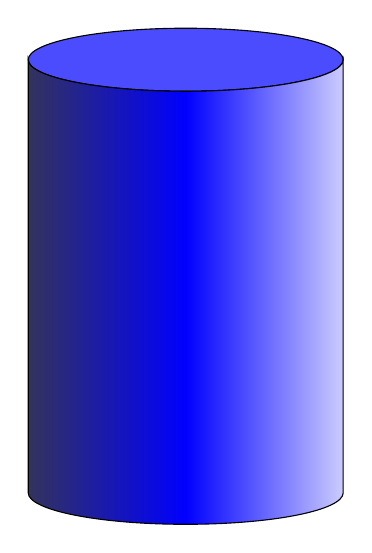
\begin{tikzpicture}
	\pgfmathsetmacro{\persp}{0.2};
	\pgfmathsetmacro{\R}{2}
	\pgfmathsetmacro{\H}{5.5}
	\def\cycol{blue}
	\filldraw[fill=\cycol!70] (0,\H) ellipse ({\R} and \R*\persp);
	\shade[left color=\cycol!20!black!80, right color=\cycol!20, middle color=\cycol,draw] (\R,0) arc (0:-180:{\R} and \R*\persp) --(-\R,\H) arc (-180:0:{\R} and \R*\persp) --cycle;
\end{tikzpicture}
\end{center}
\end{minipage}

\vspace{0.3cm}
On arrête brusquement le courant dans le solénoïde à l'instant $t = 0$ .
\begin{enumerate}
  \item Expliquer qualitativement pourquoi la charge va se mettre en mouvement à l'instant $t = 0$.
  \item Déterminer la quantité de mouvement acquise par la charge à l'instant $t = 0^+$ . On supposera
que le temps de coupure du courant infiniment court.
  \item Calculer l'impulsion du champ électromagnétique dans la situation initiale avant la coupure
du courant. On utilisera successivement les relations suivantes :
\[
\txb{grad} f × \txb{a} = \txb{rot} (f \txb{a} ) − f \txb{rot}(\txb{a})
\]
\[
\int_V d^3 \txb{r rot(a)} = \int_S d^2 \txb{s} × \txb{a}
\]
  \item Commenter le résultat de la question précédente en relation avec la question 2.
\end{enumerate}
\section{Échange de moment cinétique entre particules et champ électromagnétique}%2 
L'expérience étudiée dans ce problème, destinée à mettre en lumière la conservation du moment cinétique du système global champ + charges, est résumée sur la figure ci-dessous. Un
condensateur cylindrique $C$ , de hauteur $h$ , de rayon interne $R$ et d'épaisseur $a \ll R$ est chargé
sous une tension $U$ avec des charges $+Q$ et $-Q$ . Le tout est plongé dans un champ magnétique
constant $\txb{B} = B{\bf e}_z$ . Le condensateur se décharge alors à travers son diélectrique à partir de $t = 0$.

On négligera les effets de bord et on rappelle que dans la limite où $a \ll R$ , on peut considérer le condensateur comme plan. La capacité du condensateur et le champ électrique entre les
armatures s'écrivent alors :
\[
C = \epsilon_0\frac{2\pi Rh}{a} \ \ et \ \ \txb{E} =\frac{U}{a}{\bf e}_r \tag{1}
\]

z
B
a
R
h
Q
-Q
\begin{enumerate}
  \item Déterminer la valeur du moment cinétique $\txb{M}^i_\tx{champ}$ du champ électromagnétique avant la
décharge, en fonction de $Q$ , $a$ , $R$ et $B$.
  \item Que se passe-t-il qualitativement pendant la décharge ?
  \item Écrire l'équation donnant l'évolution du moment cinétique {\bf L} du cylindre pendant le processus. Montrer alors que, si le temps de décharge est assez court pour que le cylindre ne
bouge pas trop pendant sa mise en rotation, on peut écrire le moment cinétique final sous
la forme :
\[
{\bf L}^f = \int_Cd^3{\bf r\ r} × \int_0^\infty {\bf j}(t)dt × {\bf B}
\]
où ${\bf j}(t)$ est la densité volumique de courant.
  \item Commenter le résultat de la question précédente en relation avec la question 1.
\end{enumerate}
